\subsection{Discussion of Performance}
However, in some applications, such
as reading bank account numbers from handwritten digits, even tiny mistakes can be very costly.
Therefore, it is crucial to reduce this error as much as possible. (Raschka, 2022)

\begin{figure}[H]
    \centering
    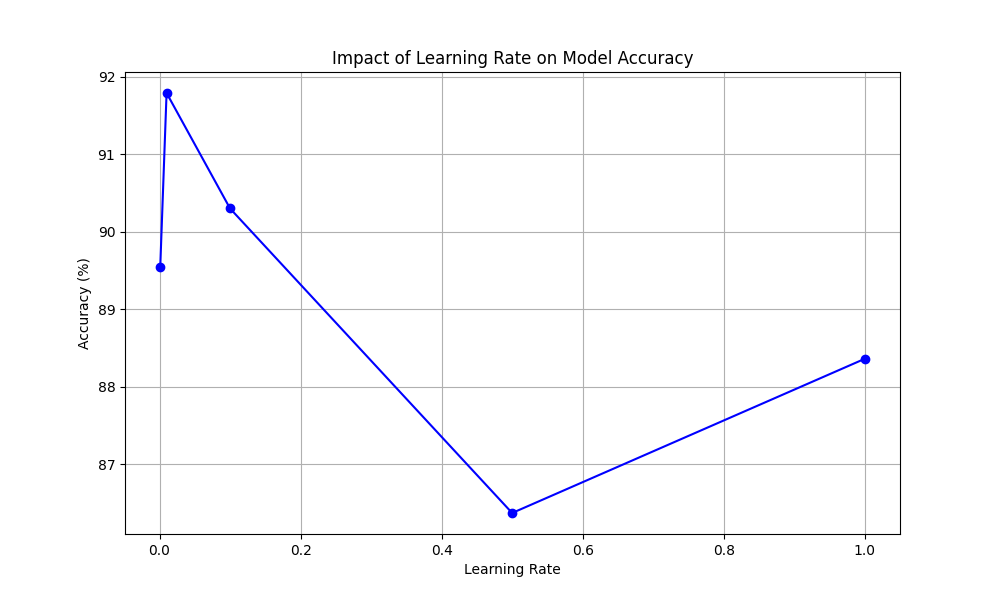
\includegraphics[width=\textwidth]{results/learning_rate_study.png}
    \caption{Logistic regression classification with learningrates in the range from $10^{-5}$ to $10^0$}.
    \label{fig:LogRegLearningRate}
\end{figure}

\begin{figure}[H]
    \centering
    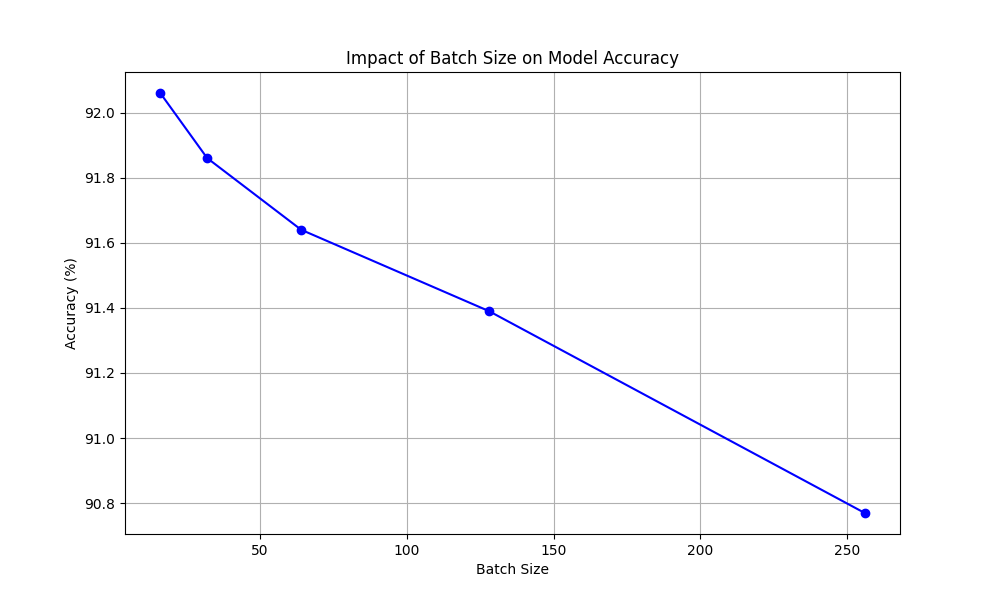
\includegraphics[width=\textwidth]{results/batch_size_study.png}
    \caption{Logistic regression classification with batchsize in the range from $16$ to $256$.}
    \label{fig:LogRegBatchsize}
\end{figure}

\begin{figure}[H]
    \centering
    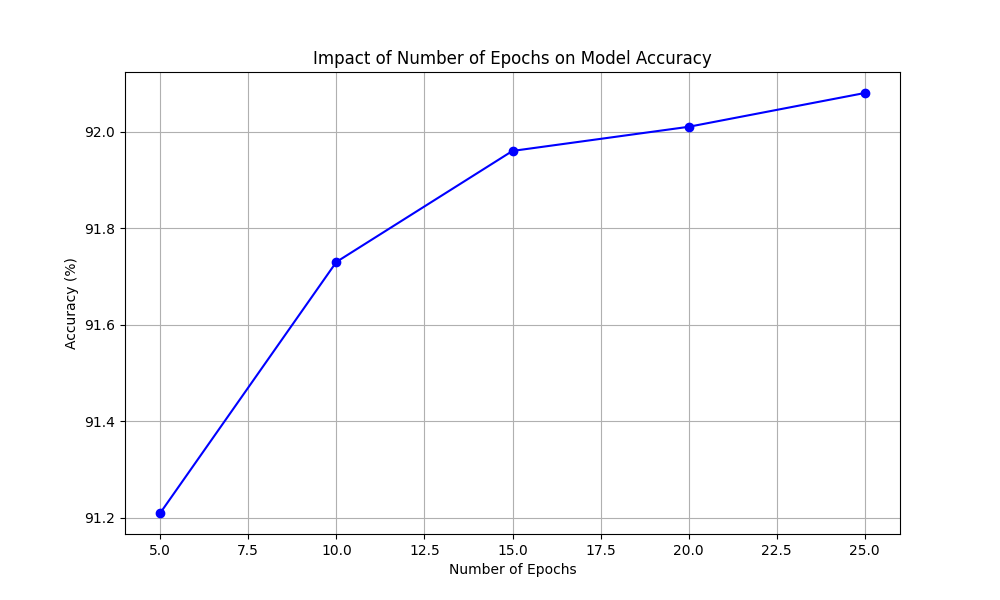
\includegraphics[width=\textwidth]{results/number_of_epochs_study.png}
    \caption{Logistic regression classification with epochs in the range from $5$ to $25$.}
    \label{fig:LogRegEpochs}
\end{figure}